\chapter*{Conclusione e lavori futuri}
Il lavoro sviluppato fino ad ora è sicuramente un punto di inizio per creare un sistema completo in grado di produrre in modo proattivo dei domini di squatting di tutte le tipologie elencate ad inizio articolo. In primo luogo bisognerebbe adattare la rete neurale ad essere in grado di auto apprendere il fatto che alcuni tipi di rumori sono utili per l'obbiettivo che vogliamo raggiungere.\\
In secondo luogo è necessario utilizzare un OCR in grado di riconoscere alfabeti differenti in modo da generare domini omografici più complessi che comprendano lettere di alfabeti differenti in quanto i domini generati e riconosciuti dalla versione attuale comprendono solo lettere dell'alfabeto inglese. Utilizzando Keras come OCR, ed essendo anch'esso una rete neurale, ho caricato i pesi necessari al riconoscimenti di lettere dell'alfabeto inglese, bisognerebbe caricare un HDF (Hierarchical Data Format) consono al riconoscimento di altri alfabeti oltre quello inglese.
Per completare il lavoro bisognerebbe aggiungere un modulo supplementare successivo all'OCR in grado di individuare quali, tra i domini riconosciuti e prodotti da SquatGAN, sono effettivamente attivi e potenziali siti di phishing. Questo sarebbe possibile farlo attraverso semplici lookup DNS.
L'architettura spiegata in figura \ref{fig:arch1} risulterebbe quindi come quella mostrata in figura \ref{fig:arch2}
\begin{figure}[!h]
  \centering
  \begin{minipage}[b]{0.6\textwidth}
    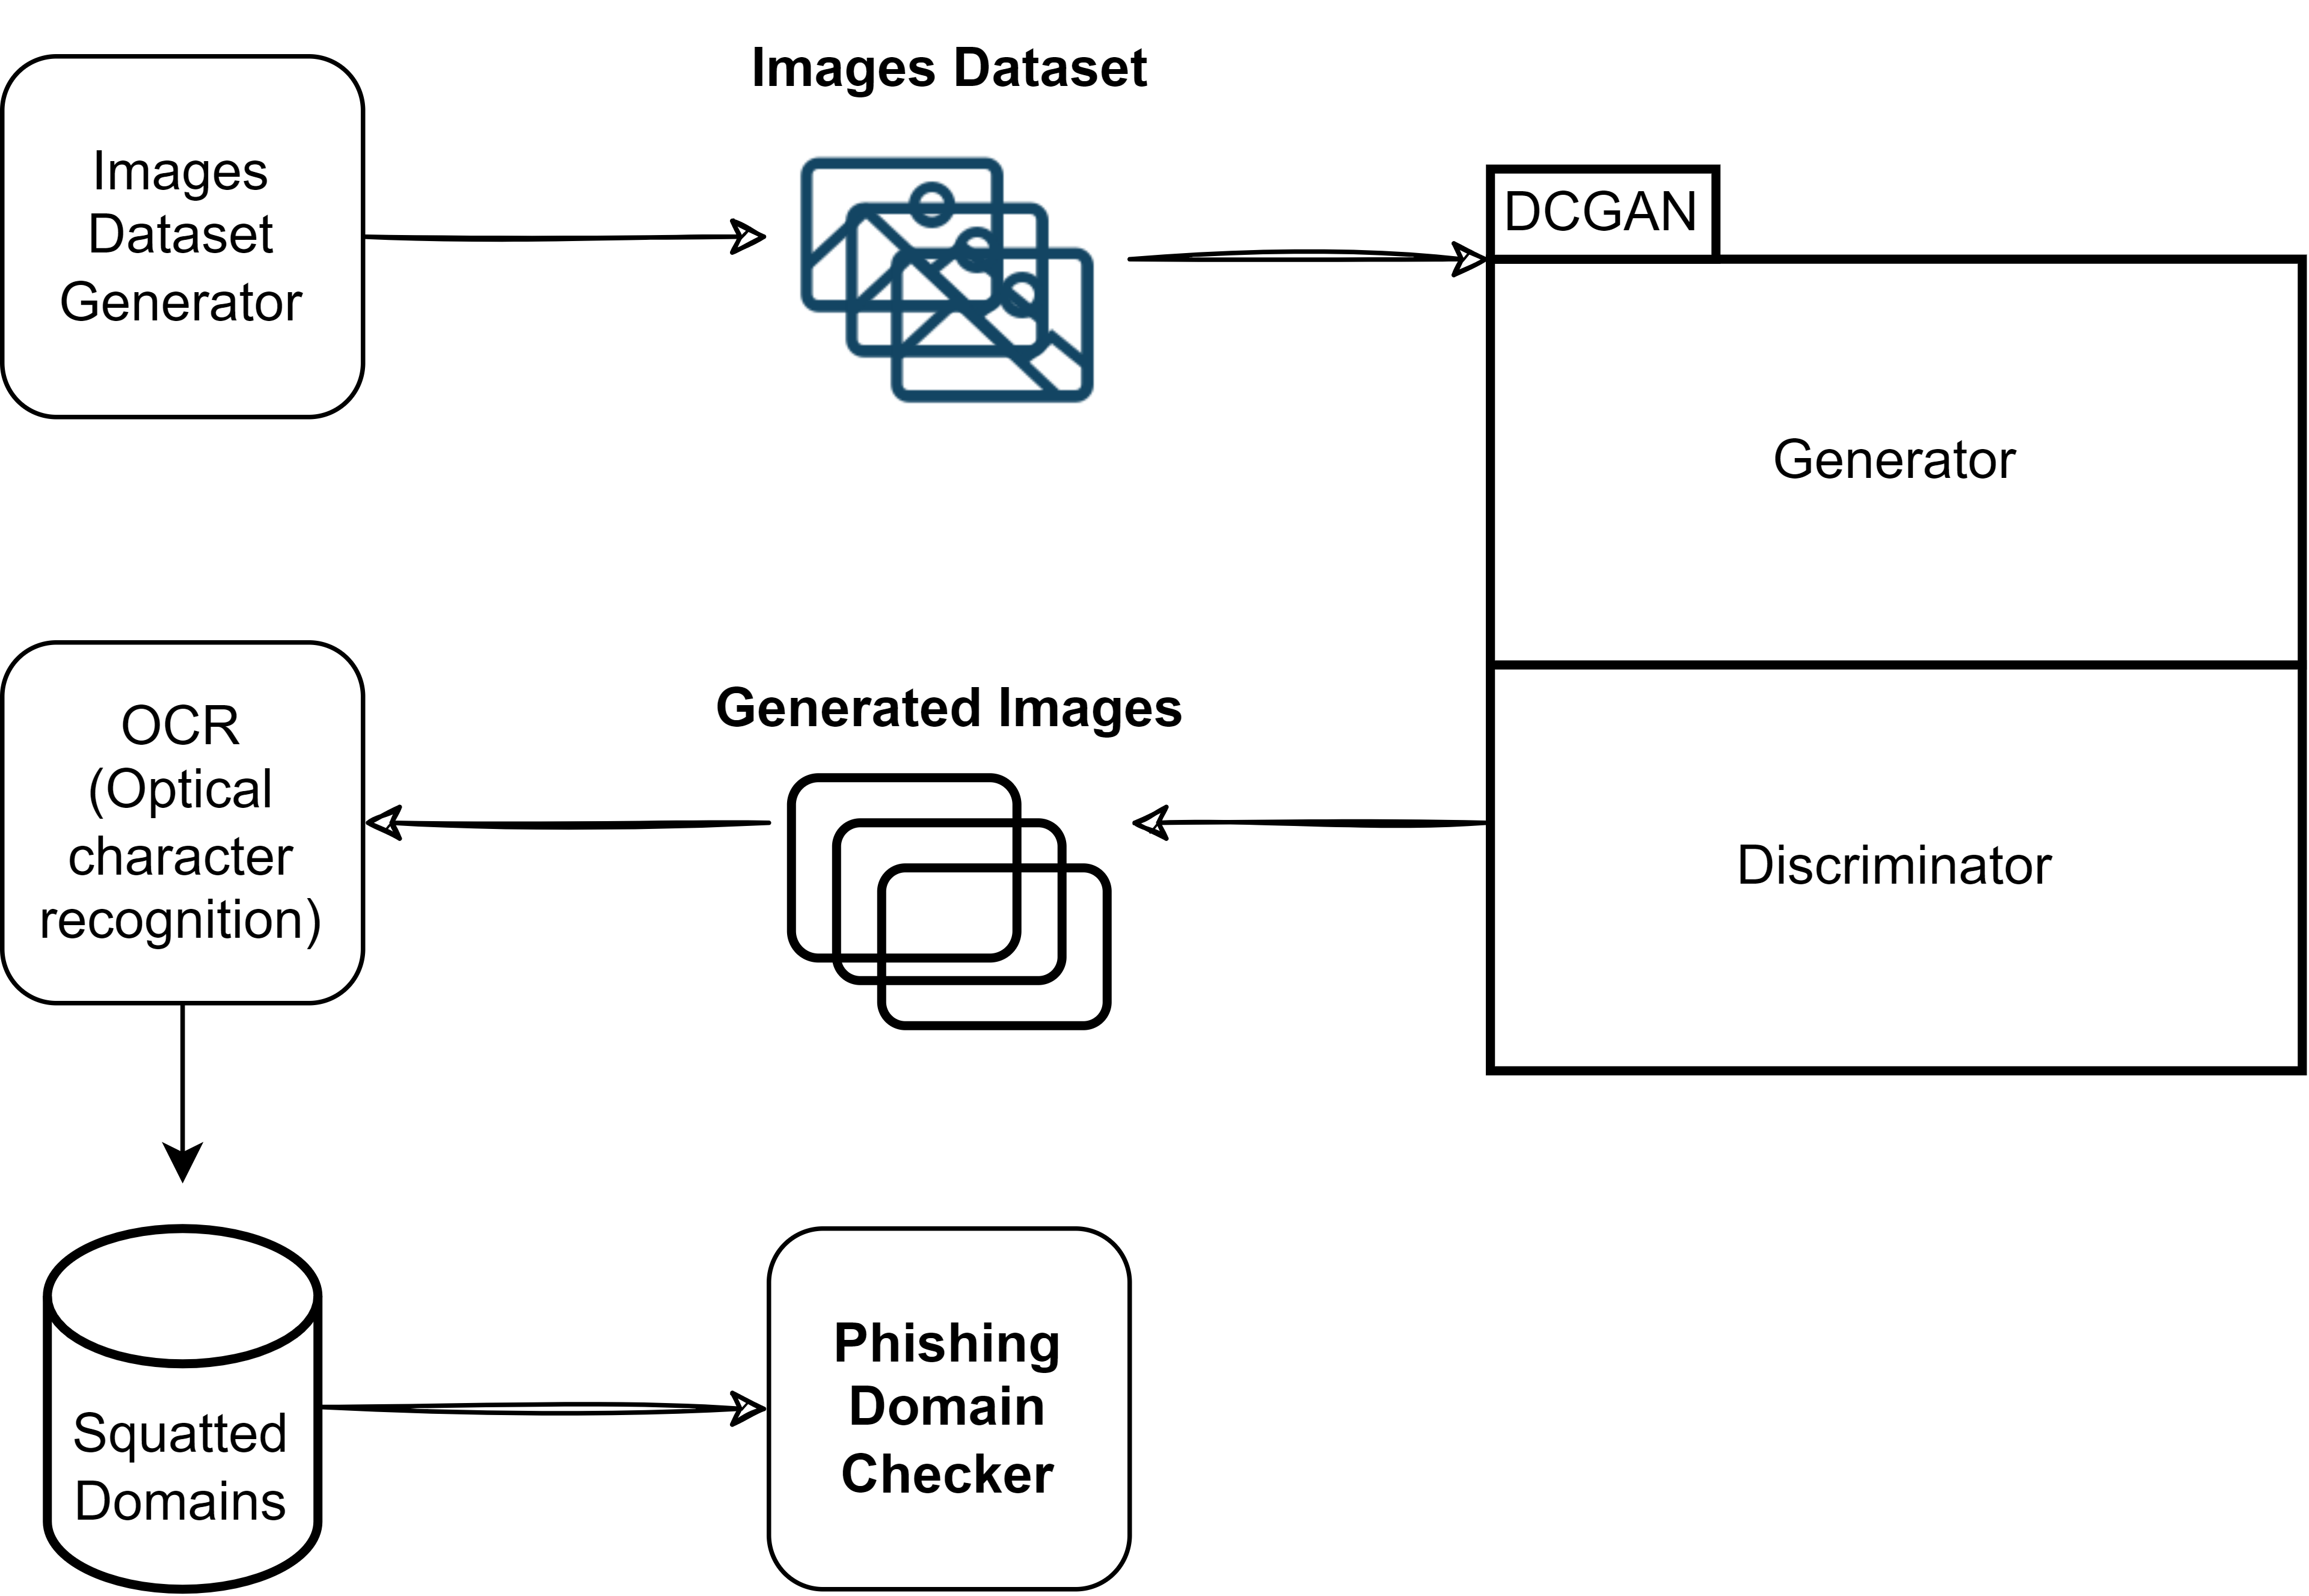
\includegraphics[width=\textwidth]{pictures/arch2.png}
    \caption{un'ipotetica SquatGAN Architecture futura}
    \label{fig:arch2}
  \end{minipage}
  \hfill
\end{figure}\\
